\section{系统分析}

\subsection{可行性分析}

本系统使用Django后端开发框架进行开发,开发环境在Ubuntu20.04操作系统下进行开发,基于Facenet的网络模型在Kaggle社区中提供的云计算平台进行训练,Kaggle社区为每个用户每周免费提供36个小时的加速计算平台,GPU硬件型号为Tesla P100,训练神经网络模型的框架使用PyTorch,以上所涉及到的编程框架以及开发环境都是开源的,所以在开发阶段并不需要投入过多的经济费用开支,而在开发完成之后的部署阶段,该系统即可选择云服务商提供的云主机进行部署,也可选择使用部署在其它服务器之上的系统。即使使用云服务商提供的云主机的方式进行部署,维护与租用费用都是完全可以接受的。从市场需求的角度来讲,现阶段大部分的中小型工厂企业所使用的的信息管理方式大多都为半手工半计算存储的方式来进行管理,使用本系统既可以解决手工管理信息的任务量大,也可以高效地对信息进行统一组织,并且将数据存储到云主机上,也可以有效防止信息丢失的问题。

\subsection{业务需求}

\subsubsection{账号注册与登录}

在用户访问首页时,首先在访问请求中查询用户是否已经登录账号,之后根据登录与否,在页面顶部导航栏中显示欢迎用语或者显示登录按钮供用户登录。在注册页面,在用户填写注册信息之后,首先在用户终端使用JavaScript检测当前输入的信息格式是否正确,通过验证后发送请求到服务后端,再根据填写的信息进行进一步验证,例如验证电子邮件是否已经存在或组织名称是否冲突等,之后在数据库的用户表插入记录,存储用户信息,当注册成功之后,自动跳转到登录页面,之后登录流程如图\ref{fig:login}所示。

\begin{figure}[H]
    \centering
    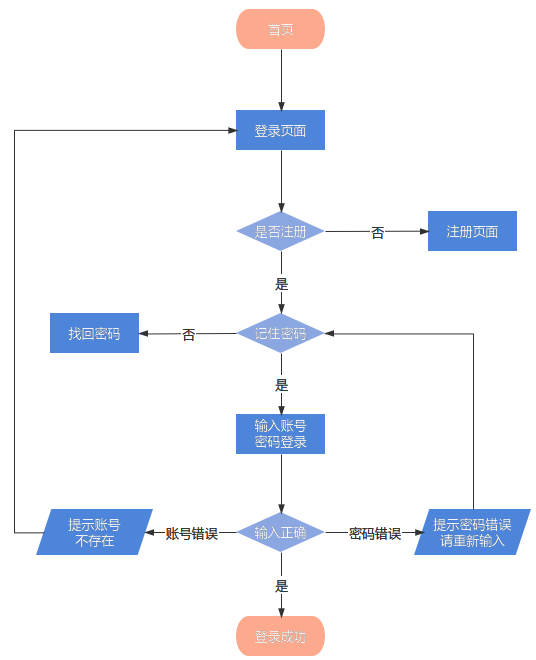
\includegraphics[width=.35\textwidth]{figures/3loginprocess.png}
    \caption{用户登录流程图}
    \label{fig:login}
\end{figure}

\subsubsection{工厂信息管理}

管理员对工厂信息进行管理时,包括交易记录、员工信息、客户信息、供应商信息、产品信息和原材料信息等。其中对员工信息进行管理时,除了员工的个人信息以外,还需要对指定员工进行下达工作任务,例如指定制作的产品、使用的原材料和生产重量等;还包括对员工的薪资进行支付等操作。在涉及到客户信息管理,除了客户个人信息之外,还需要包括对指定客户根据产品以及重量信息的下单功能进行设计。还需根据客户的订单状态,分别查看已送达的订单和未送达的订单,对订单进行管理。在对原材料信息进行管理时,还需要添加根据供应商来购入指定的原材料,由管理人员录入需要购入的价格以及重量等信息。在对员工进行考勤时,使用人脸识别对员工识别并且进行签到,将信息存储到签到表。系统的用例图如图\ref{fig:usecase}所示。

\begin{figure}[H]
    \centering
    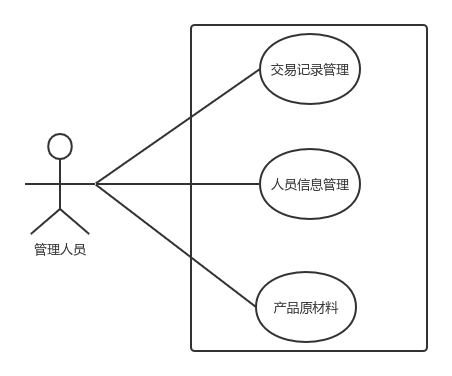
\includegraphics[width=.75\textwidth]{figures/3usecase.png}
    \caption{系统用例图}
    \label{fig:usecase}
\end{figure}

\subsubsection{人脸识别签到}

管理员对员工进行考核时,使用人脸识别对输入图像进行扫描,将根据人脸识别模块的输出对应的员工信息进行签到记录,将记录插入到员工签到表。对于人脸识别系统\cite{deepfrsurvey},有3个不可或缺的组成部分如图\ref{fig:facerec}所示。

\begin{figure}[H]
    \centering
    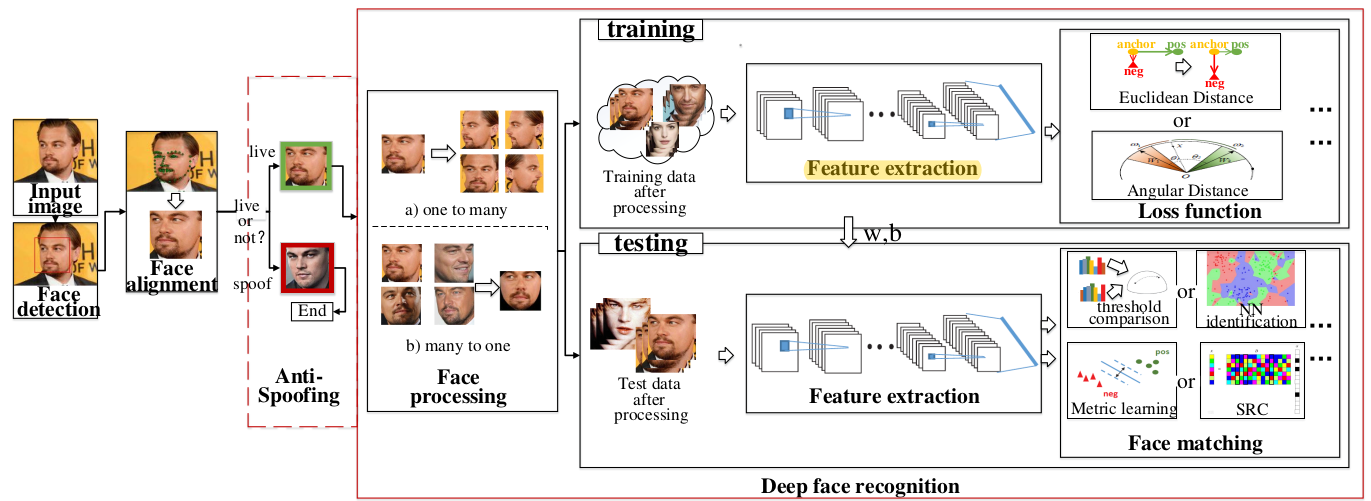
\includegraphics[width=\textwidth]{figures/3facerec.png}
    \caption{人脸识别系统组成部分}
    \label{fig:facerec}
\end{figure}

首先,使用人脸检测模块对输入的图像或视频进行人脸检测,返回当前输入的图像或视频是否存在人脸。之后使用人脸对齐模块,对输入图像中的人脸进行关键点检测,将图像中的人脸部分对齐规范到标准坐标中。将人脸对齐模块的输出图像输入到特征提取模块,通常为深度卷积神经网络进行特征提取。将提取出的特征输入到最后的人脸匹配模块,用于将当前输入的图像与人脸数据库中的图像特征进行匹配比较,通常有阈值比较、K近邻识别、指标学习和SRC等。